\documentclass{sigchi}

% Use this command to override the default ACM copyright statement
% (e.g. for preprints).  Consult the conference website for the
% camera-ready copyright statement.


%% EXAMPLE BEGIN -- HOW TO OVERRIDE THE DEFAULT COPYRIGHT STRIP -- (July 22, 2013 - Paul Baumann)
\toappear{
{\emph{University of St Andrews}}, April 10th, 2015, United Kingdom. \\
Copyright \copyright~Chi-Jui Wu. \\
}
%% EXAMPLE END -- HOW TO OVERRIDE THE DEFAULT COPYRIGHT STRIP -- (July 22, 2013 - Paul Baumann)


% Arabic page numbers for submission.  Remove this line to eliminate
% page numbers for the camera ready copy

%\pagenumbering{arabic}

% Load basic packages
\usepackage{balance}  % to better equalize the last page
\usepackage{graphics} % for EPS, load graphicx instead
%\usepackage[T1]{fontenc}
\usepackage{txfonts}
\usepackage{times}    % comment if you want LaTeX's default font
\usepackage[pdftex]{hyperref}
% \usepackage{url}      % llt: nicely formatted URLs
\usepackage{color}
\usepackage{textcomp}
\usepackage{booktabs}
\usepackage{ccicons}
\usepackage{todonotes}
\usepackage{svg}
\usepackage{amsmath}
\usepackage[toc,page]{appendix}
\usepackage{nameref}

% Set figures directory
\graphicspath{{./figures/}}
\setsvg{svgpath = figures/}

% llt: Define a global style for URLs, rather that the default one
\makeatletter
\def\url@leostyle{%
  \@ifundefined{selectfont}{\def\UrlFont{\sf}}{\def\UrlFont{\small\bf\ttfamily}}}
\makeatother
\urlstyle{leo}

% To make various LaTeX processors do the right thing with page size.
\def\pprw{8.5in}
\def\pprh{11in}
\special{papersize=\pprw,\pprh}
\setlength{\paperwidth}{\pprw}
\setlength{\paperheight}{\pprh}
\setlength{\pdfpagewidth}{\pprw}
\setlength{\pdfpageheight}{\pprh}

% Make sure hyperref comes last of your loaded packages, to give it a
% fighting chance of not being over-written, since its job is to
% redefine many LaTeX commands.
\definecolor{linkColor}{RGB}{6,125,233}
\hypersetup{%
  pdftitle={SIGCHI Conference Proceedings Format},
  pdfauthor={LaTeX},
  pdfkeywords={SIGCHI, proceedings, archival format},
  bookmarksnumbered,
  pdfstartview={FitH},
  colorlinks,
  citecolor=black,
  filecolor=black,
  linkcolor=black,
  urlcolor=linkColor,
  breaklinks=true,
}

% create a shortcut to typeset table headings
% \newcommand\tabhead[1]{\small\textbf{#1}}

% End of preamble. Here it comes the document.
\begin{document}

\title{Tracking People with Multiple Kinects}

\numberofauthors{1}
\author{%
  \alignauthor{Chi-Jui Wu\\
    \affaddr{Computer Science, University of St Andrews}\\
    \affaddr{United Kingdom}\\
    \email{cjw21@st-andrews.ac.uk}}\\
}

\maketitle

\begin{abstract}
This paper is my undergraduate thesis, completed in School of Computer Science, University of St Andrews, in 2015. The current work is a people tracking system consisted of multiple Kinects. The project aim is to track people in real world environments and resolve the occlusion problem. The final product contains an interactive software for tracking people and an user study on the developed system. The strengths and limitations of the system are discussed.

Word count: 
\end{abstract}

\keywords{Tracking; Occlusion; Kinect; Calibration; HCI}

\category{H.5.m.}{Information Interfaces and Presentation
  (e.g. HCI)}{Miscellaneous}{}{}

\section{Introduction}
\label{sec:introduction}


\section{Problem statement}
\label{sec:problem_statement}

The task of detecting and tracking moving targets in real world environment is non-trivial. There are many sources of tracking errors, such as sensor data noise and outliers, illumination levels, changing backgrounds, and occlusion. Real world environments are stochastic. Occlusion occurs when a tracked target is masked by other objects in existing fields of view. The position and movement of an occluded subject are unknown, hence increasing the difficulty of detection and tracking. Occlusions can be static and dynamic, as well as partial and full. Static occlusions refer to situations where stationary objects obstruct the visibility of the target, and dynamic occlusions occur during the interactions of many targets. Partial and full occlusion cases are when the target is partially and fully blocked from the view, respectively. THe current work attempts to resolve all different types of occlusion.

The problem is illustrated in Figure \ref{fig:occlusion_problem}.

\begin{figure}[!h]
  \centering
  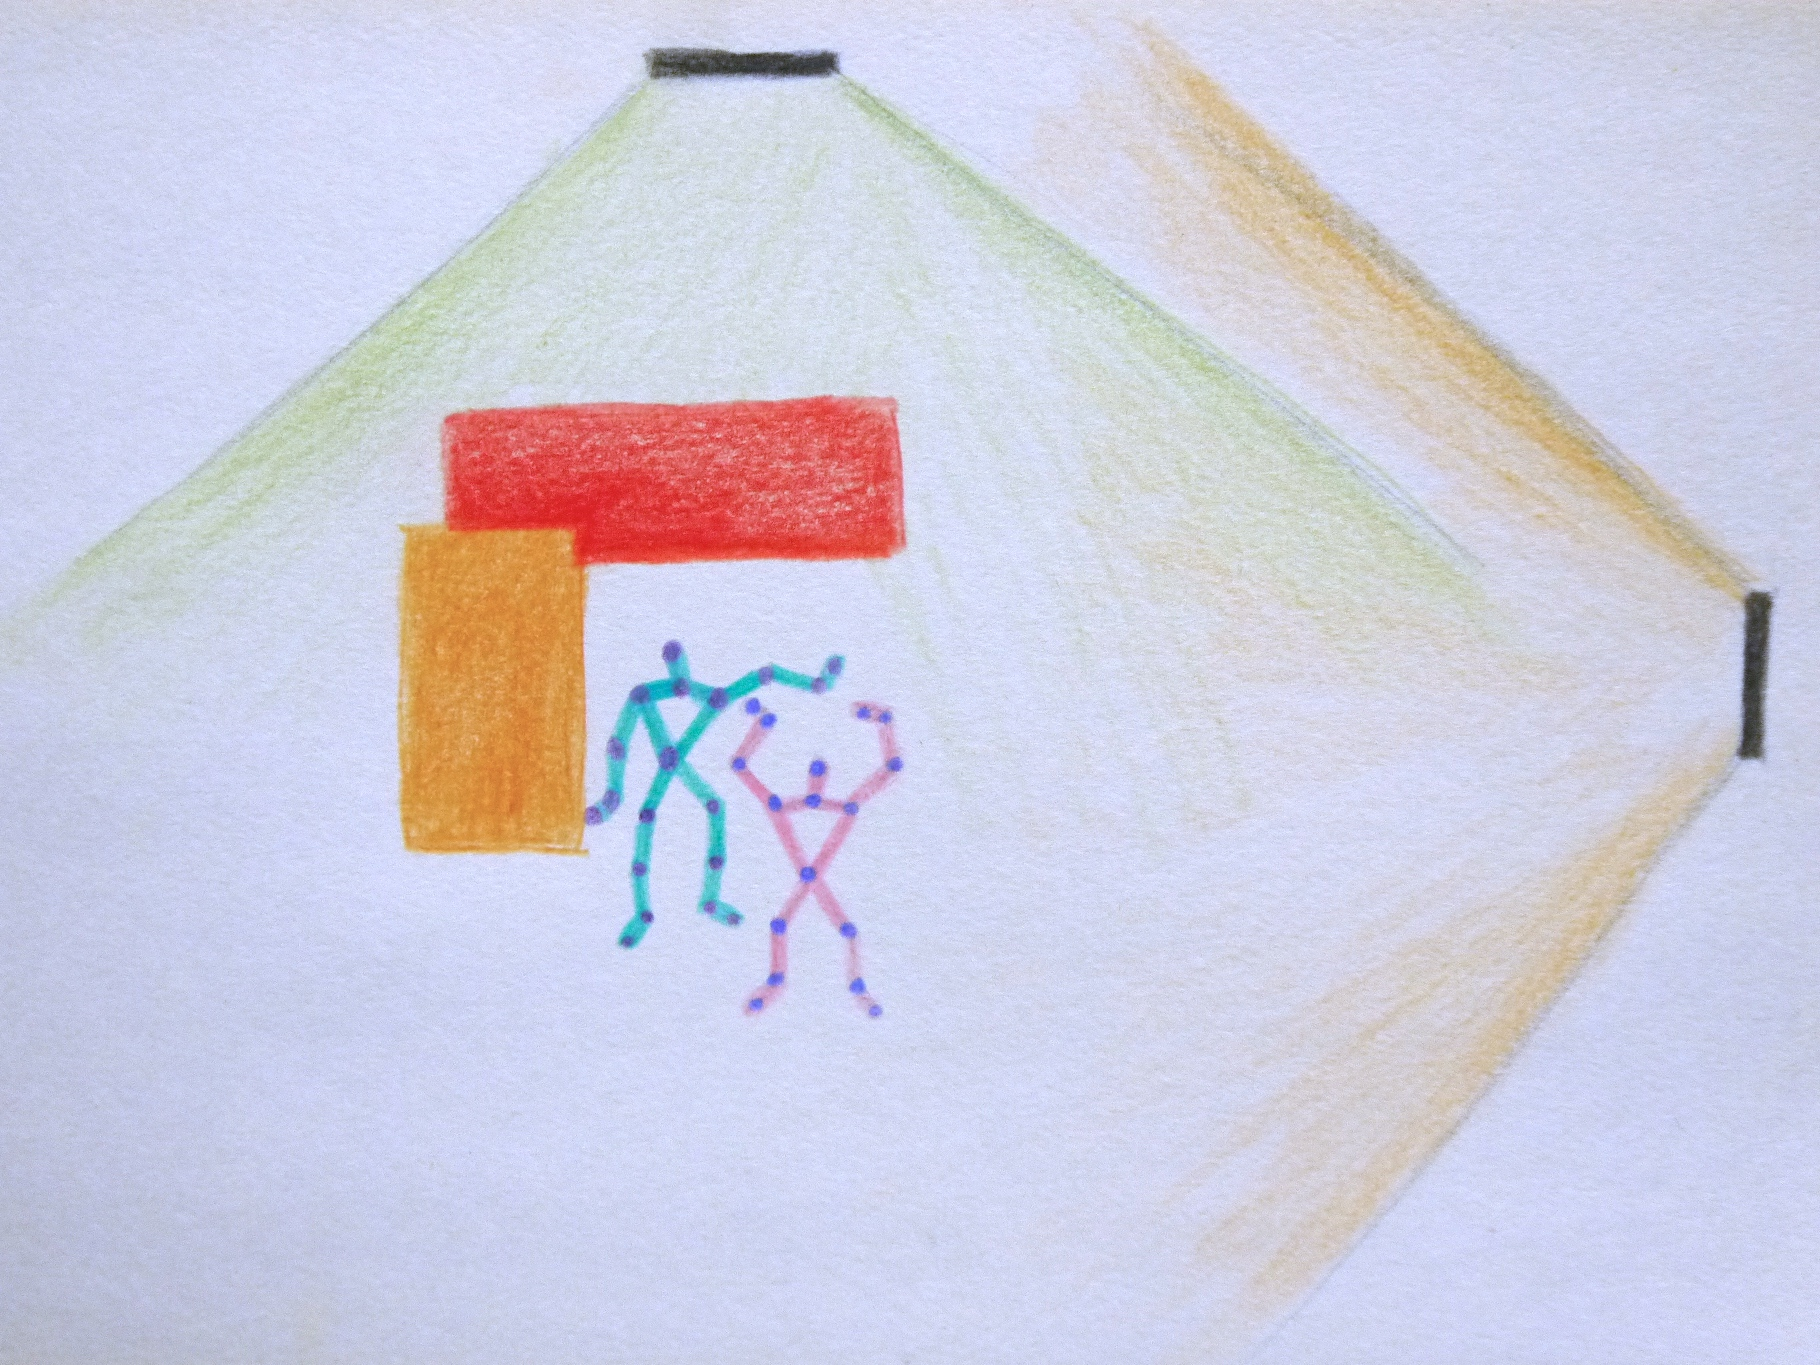
\includegraphics[width=0.9\columnwidth]{occlusion_problem}
  \caption{The occlusion problem}
  \label{fig:occlusion_problem}
\end{figure}

\subsection{Aims and Objectives}

\section{Contributions}
\label{sec:contributions}

Replicate current research, discuss limitations, (in)validate results. Resolve the problem of occlusion using multiple Kinects. 

\begin{enumerate}
  \item The first item
  \item The second item
  \item 
\end{enumerate}

\section{Previous Work}
\label{sec:previous_work}

Existing people detection and tracking techniques. Tracking people in surveillance video and in real time. Tracking using mobile and wearable devices. Motion sensors and wireless. Time-of-flight and structured-light cameras.

[Paper: Particle filter to track multiple people for visual surveillance]
[Paper: Tracking People in Video Sequences by Clustering Feature Motion Paths]
[Paper: Evaluation of real time people tracking for indoor environments using ubiquitous motion sensors and limited wireless network infrastructure]
[Paper: Tracking people under heavy occlusions by layered data association]
[Paper: Detection and Tracking of Occluded People]

\subsection{Tracking people}

\subsection{Coordinate transformation}

\cite{wei_kinect_calibration}
\cite{eggert_four_algorithms}
\cite{horn_unit_quaternions}

\subsection{Tracking using depth data}

\subsection{Tracking using color data}

[Paper: Tracking people within groups using RGB-D data]
[Paper: Detecting and tracking people in real time with RGB-D camera]
[Paper: Applications for a people detection and tracking algorithm using a time-of-flight camera]
\*[Paper: Real-time Human Motion Tracking using Multiple Depth Cameras]
[Paper: Human Detection Using Depth Information by Kinect]

\section{Kinect}
\label{sec:kinect}

The specification and components. Include image Larger field of views. Give examples.

\subsection{Features}

\subsection{Coordinate System}

Kinect Camera Space. The coordinates are 3D points (x, y, z), expressed in meters. THe origin of the coordinate system at (0, 0, 0) is at the center of the Kinect's IR sensor. The x axis grows to the left of the Kinect, the y axis grows upward, and the z axis grows outward from the direction of the sensor.

\cite{microsoft_kinect_coordinates}

\subsection{Multiple Kinects}

\section{Current Approach}
\label{sec:current_approach}

The current work is an extension on the Wei et al study \textbf{(add reference)}. It applies the same algorithms for doing calibration and coordinate transformation on the skeleton joints from different Kinects. After calibration, the system would match skeletons from multiple Kinects to form models of the tracked people. Wei et al designed and tested the system for a single user. The current system extends it to handle six people, which is the maximum number of skeletons one Kinect can recognize in its Body stream. After the calibration phase, for every new frame the system receives from the Kinects, the system would update the spatial positions of the skeletons in the corresponding models.

The system would also visualize the skeletons before and after applying coordinate transformation. The transformed skeletons are color-coded for the ease of distinguishing skeletons belonging to different people. The transformation process would inherently produce some errors, therefore, the system attempts to minimize the skeleton joint differences by constructing an average skeleton for every person.

The system is a standalone application written in C\# (.NET Framework 4.5), but it can also integrate with other applications, such as a heart rate estimation application using Kinect color data. More details on the design and implementation of the application will be discussed in section ``\nameref{sec:application}".

\subsection{System architecture}

The system topology consists of one or more machines in a client-server model. The latest Kinect v2 SDK at the time of writing (version 2.0.1410.19000) still does not support running multiple Kinects on a single machine, as a result, the system leverages the TCP/IP protocol for communicating between multiple Kinects. In the current system architecture, each client is running one Kinect (Figure \ref{fig:}). There is only one server, and any client machine can also run the server. All clients send Kinect Body frames to the server. The server is the workhorse of the system. It serves incoming client connections, establishes network streams with the clients, runs the user interface and exchanges information with the tracker (whom in runs the tracking algorithm), and lastly, informs the logger to write tracking data to files.

\begin{figure}[!h]
  \centering
  \includesvg[width=0.9\columnwidth]{system_diagram}
  \caption{An overview of the system topology}~\label{fig:system_diagram}
\end{figure}

\subsection{Clients and Servers}

The clients and servers communicate through TCP connections. The server opens the a port on the TPC network, and clients request connections to the server via sockets. When a client starts running, it will also start the Kinect \textbf{(change code: only start the Kinect after it's connected to the server)}. The client will continuously make connection requests until the server responds. If a connection is terminated by the server before the client stops running, the client will keep trying to reconnect to the server.

After the client establishes a connection with the server, it will start sending Kinect Body frames to the server. The low level networking is handled by the Microsoft .Net framework. The client serializes this data before transmitting it to the server, and the server will deserialize it. The server will then passes on the data to the tracker.

\subsubsection{Communication Protocol}

There is no initial handshaking between the client and the server. In other words, the server will accept any connection request. The server will send a confirmation message to the client after it has received the data, but the client will ignore and proceed to send the next available frame. There is minimal amount of networking

\subsection{Kinect BodyFrame}

The Kinect BodyFrame contains information about the people that are tracked by the Kinect sensor in real time. It was called the SkeletonFrame in the Kinect v1 SDK. Each frame contains at most six Kinect Body data, where each Kinect Body represents an actively tracked or inferred skeleton. A Kinect Body stores the joints coordinates and their metadata. These information are computed by the Kinect sensor from its depth data. The current system uses the preprocessed information for tracking individuals.

\subsubsection{Serialization}

The Kinect v2 SDK does not support serialization of the Kinect BodyFrame. The current work builds a Kinect BodyFrame serialization library for transmitting this data across the network. See the appendix for a complete list of serialized properties. Among all the serialized data, the most important pieces of information are the skeleton joints, their position in the Kinect Camera Space, the type and the tracking state of each joint.

\subsection{Calibration}

The server passes on the Kinect BodyFrames to the tracker, who initiates the calibration process. The system performs calibration to ensure that people's initial position and angle are taken correctly. The initial position is defined as the average coordinate of all visible joints coordinates from the skeleton. The initial angle is defined as the the angle between the Kinect and the skeleton. The mathematical formulae can be found in \textbf{(todo: insert pseudocode)}. Subsequently, they can be used as reference points during coordinate transformation. The tracker will initiate the calibration process once it has received sufficient frames from all connected clients, or Kinects.

The initial angle $\theta$ has three different cases. It is zero when the center of the skeleton is perpendicular to the sensor. It is positive when the skeleton is facing right, or left of the sensor. Lastly, it is negative when the skeleton is facing left, or right of the sensor.

\subsubsection{Procedure}

The calibration procedure is replicated from the method proposed by Wei et al, with minor adjustments. The system uses 120 Kinect BodyFrames for calibration, which takes four seconds, because Kinect sends the BodyFrame at 30 frames per second. If there were more frames available from any connected Kinect, the tracker would use the most recent frames. All calculations performed during calibration are done using the Kinect Camera Space.

\subsubsection{Detecting interference}

The tracker will automatically initiate recalibration if people move their joints over ten centimeters \textbf{(todo: insert pseudocode)}. The current implementation checks movements at a person's head, left hand, and right hand.

\subsection{Coordinate transformation}

After the tracker completes calibrating the Kinect coordinate system, it can transform any joint of a skeleton to a world coordinate. Joints in the world coordinate system can be transformed back to any Kinect field of view. Tracker uses the joint coordinates in world view to find skeletons belonging to the same person in different Kinect fields of view. When tracker finds all skeletons of the same person, it can transform all corresponding joints in world view to a single Kinect's camera space, showing combined depth sensor information for the tracked person. The transformation process is the very first step in filling the missing joints, hence the whole body, in the average skeleton during occlusion. Unsurprisingly, the effectiveness of the system depends heavily on how accurate the transformation is done.

\subsection{Tracking by detection}

After calibration, all the tracker sees is a collection of skeletons with their initial position and angle. As aforementioned, the tracker can represent these skeletons in both the Kinect Camera Space and the world coordinate system. This information is not useful on its own, and the more people there are in the views of the Kinects, the larger this collection of skeletons would be. The tracking system should know which skeletons belong to which person, thus knowing about people's absolute position relative to any Kinect field of view.

The tracker construct models of tracked people by finding skeletons in different fields of view that have high proximity in the world coordinate system. The tracker performs the detection algorithm using joints in the world coordinate system, because using these coordinates would allow the tracker to compare skeletons' spatial positions regardless of perspectives. It assumes that skeletons from different Kinects field of view that have the highest proximity must belong to the same person. The tracker continues this process until it can no longer put skeletons in pair. The pseudocode is shown below \textbf{(todo: insert pseudocode)}.

The current implementation assumes that every person is visible to all Kinects. The system works fine when there is only one person who is occluded from all Kinects, because the person would only have one skeleton, leaving it to the last to be matched. The system would not detect people correctly in scenarios where several people are occluded from all Kinects in the calibration phase, because it would try to match skeletons from different Kinect fields of view even though they are far apart from each other. \textbf{(todo: add illustrations of a working scenario and a non-working scenario)}.

Every calibration process follows a people detection result. It entails models of currently tracked people, where each model consists a number of potential skeletons, all from different Kinect perspectives. A potential skeleton represents one replica of a person from a Kinect field of view. The average skeleton of a person is the average body across all potential skeletons in the person's model. The average skeleton of a person can be seen as the system's view of that person. The result is permanent until the system recalibrates. That is, the same skeletons are always associated with the same person whom they were initially identified with. 

The system performs tracking by updating every potential skeleton in the current result, propagating the changes to the skeleton visualization.

\subsection{Detecting occlusion}

When a person obstructs another person causing a Kinect sensor to partially or completely lose the sight of the masked person, the system would fill in the joints from other actively tracked potential skeletons. The average skeleton would be calculated using only the actively tracked joints from all potential skeletons. The effect would be visible on the application front-end; the visualization would display the latest average skeleton.

\subsection{Detecting new and missing people}

The system makes the assumption that people during calibration will be the only people in the scene throughout the lifetime of the system. This is because the system does not have any information about the new people entering the scene that would otherwise be obtained during calibration, such as their precise initial position and angle, which are needed to perform coordinate transformation. When the system detects intruders or zero people in the scene, it would automatically initiate calibration. \textbf{(todo: finish coding)} Scenarios where a number of skeletons, but not all, is missing from the system's available Kinects are unimportant, because the people possessing those skeletons may only be temporarily occluded.

Since the positions of all potential skeletons are updated every frame, the system would know when the skeletons are missing. The scene is empty if and only if every potential skeleton in the scene is empty.

\subsection{Strengths}

\subsection{Limitations}

\subsection{Improvements}

\section{Application}
\label{sec:application}

The final application demonstrates that the system works as intended. The main components of the application consist of a server, a tracker, a user interface, and a logger. The server passes on the Kinect BodyFrames received from the clients to the tracker. The tracker then processes the data and signals the user interface when the latest result is available. The user interface displays the tracking result on the skeleton visualization. When required by the end user, the logger would write tracking result to files.

\begin{figure}[!h]
  \centering
  
\includegraphics[width=0.9\columnwidth]{ui}
  \caption{UI}
  \label{fig:ui}
\end{figure}

\subsection{Running the application}

\subsection{Design}

The application should be intuitive and easy to use. Since it is a prototype demonstrating the capability of the tracking system, it puts large emphasis on the skeleton visualization, showing that the combined skeletons match the expected outcome of the tracking process. The application displays the skeletons before and apply applying coordinate transformation and skeleton matching. The combined skeletons should render at the same speed as the server receives BodyFrames from multiple sources. 

The application provides the end users essential functionalities for running the application, including start and stop the server, recalibrate, view tracked skeletons from different views, and send the average skeleton stream to other applications. The user interface will fire a ``OnDisplayResult'' event when the rendering of the skeleton visualization is completed. This lets the server know when to signal the logger.

The overall control flow of the application is now clear. The server handles data from the clients. The tracker processes the data. The user interface visaulizaes the data and provides additional control for the user. If required, the server then tells the logger to store the tracking done after the visualization is shown.

\textbf{(todo: implement recalibration and stop button and the last feature)}

The application does not take the following elements into design decision:

\begin{itemize}
  \item The security of the application.
  \item The privacy of users' tracking information
  \item The scalability and robustness of the server.
\end{itemize}

\subsection{Client Implementation}

\subsection{Server Implementation}

The application is written in C# with the .NET 4.5 framework, and the user interface is created using the .NET WPF framework, because the official Microsoft Kinect SDK is written in C# and the latest examples use the WPF framework. 

The application leverages the C# events and delegates model. The application components subscribe to the event queues of other components. When new data is available from the subscribing component, the subscribed component consumes the data, does something with it, and fires events to all of its subscribed components. The components on the receiving end do the same, and so on. The server aseembles the overall communication via events.

The application is started with one parameter, the server port number. It then creates a server to be run at that port number. The server will only start running when it receives such command from the user. After the server is created, it creates the user interface thread as a Single Threaded Apartment running in the background. The user interface will appear now.

\subsubsection{Events}

The server will receive the following events from the user interface:

\begin{itemize}
  \item Setup parameters for the server
  \item Start the server
  \item Stop the server
  \item When the user interface has displayed the tracking result (then the server will notify the logger)
\end{itemize}

The user will have control over the server, hence the system.

The server will pass the following events to the user interface:

\begin{itemize}
  \item Clients (Kinects) have been connected to the server
  \item Clients (Kinects) have been removed from the server
\end{itemize}

The user interface can know which Kinects are connected to the server, giving the user feedback and later allowing him to choose from which Kinect perspective to view tracked people's skeletons.

The server will bind the following events from the tracker to the user interface:

\begin{itemize}
  \item The tracker is waiting for Kinects to be connected
  \item The tracker is calibrating (and how many frames remaining)
  \item The tracker needs recalibration (and for what reason)
  \item The tracker has synchronized the latest BodyFrame with the tracking result 
\end{itemize}

The user interface would show more feedback, including the latest result, from the tracker.

\subsubsection{Server}

The application listens for TCP client connections. This work is done in a separate thread, called the ServerWorkerThread. When the TCP socket listener receives a new connection, the server will handle it in a new, separate thread. In the socket thread, the server will create a network stream between the client and the server. After the connection is established, the server will fire a ``OnKinectConnected'' event to the user interface. Later on, the server will receive Kinect BodyFrames from the client through the network stream it had created. Upon receiving some data, the server would deserialize it into a BodyFrame object, then it would fire another event called ``Track'' to the tracker with information about the sender and the BodyFrame itself. Lastly, the server will send a response (a string) back to the client. The response is trivial; it is used to tell the client that the data has been received. The client is also implemented so that it In the current implementation, the server returns ``Okay''. The server will continue to process additional BodyFrames received on its end of the netwrok stream, and the above procedure repeats.

\textbf{(todo: fix the server so that it can stop and report the additions)}

\subsection{User Interface Implementation}

The application has one window. It has a number of small buttons as controls on the top of the interface. Below the controls the window is split into halves. The left hand side shows the visualization for merged skeletons after applying coordinate transformation, and the right hand side shows the visualization of skeletons in their original fields of view. Displaying the two different views at once demonstrates the system's tracking algorithm.

The design decisions on the look of the user interface are not discussed, because aesthetic features were not taken into consideration when the user interface was developed.

\subsubsection{Controls}

Available user controls are shown as buttons. The user interface responds to click events on each button. Buttons representing functionalities are that not meant to be used are disabled. For instance, when the start button is pressed, signaling the server to start running, the setup button, which parameterizes the server, should be disabled. A full set of constraints on the availability of the buttons are specified below:

\textbf{(todo: should I put this down?)}

\subsubsection{Events}

When the user interface receives events from the server about new and old connections with clients, the user interface adds and remvoes option to transform the kinect Bodies into the particular Kinect's field of view, respectively. The user interface would also display texts, centered on the left hand side visualization, about the progress of calibration or any interrupted action causing calibration to fail. How the user interface displays the BodyFrames is discussed in the next subsections  ``\nameref{subsec:tracking_view}'' and ``\nameref{subsec:disjoined_view}''.

\subsubsection{Tracking View}
\label{subsec:tracking_view}

The Tracking View shows the skeleton visualization of the tracking result. The merged skeletons are drawn from the perspective of the selected Kinect, specified by the user or is defaulted to the local client's Kinect (The local client is the client that is also running on the server machine). The average skeleton is calculated at this stage. The potential skeletons of a person share the same color, and the average skeleton is always colored white. There are six avaialble colors, because the system sets the cap of number of tracked people to six.

The skeleton visaulization in both Tracking View and Disjoined View has the same implementation. The bones of the skeletons are drawn first, then the joints. The simplified list of human bones using the Kinect joints are taken from the Microsfot Kinect Developer examples. The inferred bones are displayed thinner than the tracked bones.

\textbf{(todo: default to local Kinect)}

\begin{figure}[!h]
  \centering
  \includesvg[width=0.9\columnwidth]{tracking_view}
  \caption{The Tracking View}~\label{fig:tracking_view}
\end{figure}

\subsubsection{Disjoined View}
\label{subsec:disjoined_view}

The Disjoined View shows the skeleton visualization of the tracked skeletons in their original Kinect coordinate system. The skeletons are colored with respect to their Kinect origin. In other words, skeletons coming from the same Kinect would share the same color. The number of available colors is also limited to six.

\begin{figure}[!h]
  \centering
  \includesvg[width=0.9\columnwidth]{disjoined_view}
  \caption{The Disjoined View}~\label{fig:disjoined_view}
\end{figure}

\subsection{Tracker Implementation}

The tracker runs the tracking algorithm on the Kinect BodyFrames from multiple Kinects. It is the brain of the application and the system, hence the most complex. There are no generic data structures in the whole application except the tracker. 

\subsection{Logger Implementation}



\textbf{``Disjoined'' or called something else}

\subsection{Integration with Heart Rate Monitoring}

\section{Testing}
\label{sec:testing}

The system running multiple Kinects is verified by looking at the skeleton visualization on the user interface for a number of different users and in various interaction scenarios. The researcher is interested in whether the application has accomplished the following tasks:

\begin{enumerate}
  \item The skeletons from different Kinect fields of view are matched correctly to the corresponding persons in the scene.
  \item The transformed skeletons of the same person are close together, showing minimal differences in the joint coordinates.
  \item The skeletons can be transformed to different Kinects' Camera Space (3D coordinate system) for viewing
  \item All of the above statements hold when the users move freely.
\end{enumerate}

It is worth noting that the best tracking results, which minimize overall differences in joint coordinates, are when the Kinects are placed parallel to the ground floor with near 0 degree tilting angle. The researcher then investigates the performance of the tracking algorithm with the aforementioned contraints in various artificial scenarios. See the sections on User Studies for more details and the section on Future Work for improving the current system.

\subsection{Occlusion}

The main goal of the project is to show persistent tracking results in occluded environments and scenarios where complex human interactions are in play. The researcher has verified this requirement by partially and fully obstructing users in the scene. In the simplest case, a person may be self-occluded if he stands in a position such that one Kinect cannot fully see all the joints but two Kinects combined can have a complete view of the person. \textbf{(todo: show an illustration)} The research stands back-facing the main Kinect, while showing his right arm only to the second Kinect. The system would form the average skeleton using the actively tracked information from both Kinects; the average skeleton would contain joint coordinates that both Kinects are most sure about.

\textbf{todo: show different cases where the system is working properly, with images}

\section{User studies}
\label{sec:user_studies}

A series of user studies are designed to evaluate the system's accuracy at tracking people in different scenarios. The accuracy of the tracking algorithm, or essentially the coordinate transformation algorithm, is measured by the differences in the joint coordinate between multiple potential skeletons of the same person. The studies will require participants to move around in front of multiple Kinects alone and with other participants. The software will log participants' positions from tracking, and these data will provide a quantitative feedback on the accuracy of the algorithm in different Kinect configurations and user scenarios.

To reiterate, a potential skeleton is a skeleton from a single Kinect field of view. One person may have multiple potential skeletons when they are visible to many Kinects. The application is most useful for its ability to transform any potential skeleton into any Kinect's camera space. The potential skeleton in the current Kinect field of view would be unaffected, but the other potential skeletons that were in other Kinects fields of view would have slight deviations in their joint coordinates. The user studies attempt to capture such deviations in all possible cases.

Figure \ref{fig:studies_example}

\begin{figure}[!h]
  \centering
  \includesvg[width=0.9\columnwidth]{studies_example}
  \caption{A participant doing the experiment}~\label{fig:studies_example}
\end{figure}

\subsection{Hypotheses}

The null hypotheses are as follows:

\begin{enumerate}
  \item The differences in each joint coordinate among all potential skeletons of a person are consistent across time and are within five centimeters
  \item The differences in each joint coordinate among all potential skeletons of a person are consistent with different Kinect configurations
  \item The application would fill in the missing joint coordinates of a person from information about all potential skeletons
\end{enumerate}

\subsection{Apparatus}

The current studies use two machines and two Kinects. Each machine is connected to one Kinect and runs a client sending Kinect BodyFrames to the server. The server is running on one of the client machines.

\subsubsection{Computer Specification}

The server machine is running Microsoft Windows 8 on a i5 processor and 8 Gb RAM \textbf{(todo: add details)}. The other client machine is also running Microsoft Windows 8, on a i7-3610QM CPU at 2.30 GHz and 8 GB RAM.

\subsubsection{Kinect Specification}

The sensors are the v2 Kinects for Xbox One. The SDK running those Kinects is version 2.0.1410.19000.

\subsection{Participants}

Participants are multinational university students and staff. There are participants in both genders and with a wide range of heights and weights. They are compensated with chocolates for participation.

\subsection{Setting}

The studies take place in a semi-controlled environment (See Figure \ref{fig:studies_setting}). The two Kinects are placed at either three pre-defined locations, where they are approximately parallel, 45 and 90 degrees apart. One Kinect is always placed at the front position; it is the Kinect on the left in the image. (\textbf{(todo: measure the exact angles and distances between them - they are marked by duct tapes so shouldn't be too hard)}) Duct tapes are used to mark the precise locations of the Kinects. The boundary within which the participants will be moving is also marked with duct tapes. The sides of the block are found empirically to be near the minimum distance of the Kinect viewing range of the full body skeleton. The dimension of the boundary is x by x meters (\textbf{(todo: find the dimensions in meters)}). Each potential step is marked with duct tapes colored in a hue (either black or red) different from that on the duct tapes in the previous step. The starting position has a distinct color (green) from all other steps.

\begin{figure}[!h]
  \centering
  \includesvg[width=0.9\columnwidth]{studies_setting}
  \caption{The setting where the user studies took place}~\label{fig:studies_setting}
\end{figure}

\subsection{Method}

Firstly, participants are introduced to the project aims and objectives. They are given sufficient time to ask questions and decide whether to participate in the experiment before signing the consent form. Participants are free to withdraw from the studies at any time without any explanation. Secondly, participants are told beforehand what instructions they would expect during the experiments. This is because the studies are designed to measure how well the system tracks people, not how participants react to some situations. In user studies mode, the application would show instructions on the right hand side of the screen, telling the participants where to put their feet next. For instance, it would tell the participant to move forward (See Figure \ref{fig:studies_instruction}). The application will try to log as least amount of stationary movements as possible for tasks where they require participants to be moving. Not only because testing for differences in joint coordinates when the participant remains stationary is a standalone study, but also the researcher is interested in how the tracking algorithm performs when tracked people are constantly moving. To achieve this goal, the application introduces pauses between tasks. The researcher has control over the starting time of the next task. During the pauses, the researcher would give additional details about the studies to the participants.

\begin{figure}[!h]
  \centering
  \includesvg[width=0.9\columnwidth]{studies_instruction}
  \caption{Instructions during the user studies}~\label{fig:studies_instruction}
\end{figure}

\subsection{Ethics}

There are no legitimate ethical concerns about participating in the studies. The skeleton data are anonymized and will be stored up to a maximum of three years. Any participant who feels uncomfortable with the guideline is welcome to speak to the researcher and his supervisor.

\subsection{Study 1: Stationary}

In the first study, participants are required to remain stationary for ten seconds in the center of the block. The study is done with all three Kinect configurations.

\subsection{Study 2: Basic Movements}

The second study requires the participants to move in the same way as explained in the Wei et al study. These are basic movements such as moving forward, backward, left, and right. The study is done with all three Kinect configurations.

\subsection{Study 3: Continuous Movements}

The third study requires the participants to walk around the perimeter of the block and walk diagonally to each of four corners. Like the previous two studies, study 3 is done with all three Kinect configurations. Studies 1, 2, 3 are conducted in succession for every participant.

\subsection{Study 4: Two people Cross-over}

The fourth study involves two people. They stand next to each other. The person on the left will walk to the front of the other person, then back to his initial position. Then he will walk around the person, from the front to the back, then return to his starting position. The other person does the same. In the end, both people exchange positions.

\subsection{Study 5: Interaction 2?}

\subsection{Study 6: Occlusion}

Participants are asked to walk around a large obstacle, which is a large poster in the current study. The obstacle divides the field of view of two Kinects at 90 degrees apart (See Figure \ref{fig:studies_obstacle}). The participant starts on the right hand side of the obstacle, where he is visible to both Kinects. As the participant walks around the obstacle, from the back, then to the left side of the obstacle, the Kinect that was looking at the side of the participant will slowly lose the sight of the person. When the participant is on the other side of the obstacle, only the front-facing Kinect will have sight of the person. The study should demonstrate that the system would still be able to track the person despite that one of the Kinect loses the person's sight temporarily. The study is only done with Kinects placed 90 degrees apart.

\begin{figure}[!h]
  \centering
  \includesvg[width=0.9\columnwidth]{studies_obstacle}
  \caption{The obstacle in the actual experiment}~\label{fig:studies_obstacle}
\end{figure}

\section{Evaluation}
\label{sec:evaluation}

Discuss results. Compare them with Wei et al.

\begin{figure}[!h]
  \centering
  \includesvg[width=0.9\columnwidth]{stationary_p0_d7_all}
  \caption{One person all joints}~\label{fig:one_person_all}
\end{figure}

\begin{figure}[!h]
  \centering
  \includesvg[width=0.9\columnwidth]{stationary_p0_d7_average}
  \caption{One person average}~\label{fig:one_person_average}
\end{figure}

\begin{figure}[!h]
  \centering
  \includesvg[width=0.9\columnwidth]{scenarios}
  \caption{All scenarios}~\label{fig:scenarios}
\end{figure}

\section{Future Work}
\label{sec:future_work}

\subsection{User studies}

\subsection{Application}

\section{SH Project Reflection}

SECTION

\subsection{Requirements}

\section{Acknowledgements}
\label{sec:acknowledge}

I declare that, unless otherwise stated, the work is completed by myself, Chi-Jui Wu, under the supervision of Dr. David Harris-Birtill. The code for skeleton visualization is written based on the official Microsoft Kinect Developer example.
In addition, all infographics, excluding real-life images, are created by Ching Su. I retain the copyright of this work.

\balance{}

\bibliographystyle{SIGCHI-Reference-Format}
\bibliography{report_bib}

\begin{appendices}

\chapter{Glossary}

\begin{description}
  \item[First] The first item
  \item[Second] The second item
  \item[Third] The third etc \ldots
\end{description}

\chapter{Kinect BodyFrame Serialized}

BodyFrame, Body, Joint. The important elements are the tracking state, joint type, amd camera space point.

\cite{microsoft_kinect_namespace}

\end{appendices}

\end{document}
